% ---------------------------------------------------------------------------
% ---------------------------------------------------------------------------
% Junção de templates encontrados no Overleaf
% facilitando a vida do aluno de pós da UFABC
% Modelo LaTex para preparação do documento final de Dissertação de Mestrado
% ninguém do programa de pós da informação validou se presta
% ---------------------------------------------------------------------------
% ---------------------------------------------------------------------------

\documentclass[
	% -- opções da classe memoir --
	12pt,					% tamanho da fonte
	openright,				% capítulos começam em pág ímpar (insere página vazia caso preciso)
	twoside,					% para impressão em verso e anverso. Oposto a oneside
	a4paper,					% tamanho do papel. 
	% -- opções da classe abntex2 --
	%chapter=TITLE,			% títulos de capítulos convertidos em letras maiúsculas
	%section=TITLE,			% títulos de seções convertidos em letras maiúsculas
	%subsection=TITLE,		% títulos de subseções convertidos em letras maiúsculas
	%subsubsection=TITLE,	% títulos de subsubseções convertidos em letras maiúsculas
	% -- opções do pacote babel --
	english,					% idioma adicional para hifenização
	%french,					% idioma adicional para hifenização
	%spanish,				% idioma adicional para hifenização
	brazil					% o último idioma é o principal do documento
	]{abntex2}

% ---------------------
% Pacotes OBRIGATÓRIOS
% ---------------------
\usepackage{lmodern}				% Usa a fonte Latin Modern			
\usepackage[T1]{fontenc}			% Selecao de codigos de fonte.
\usepackage[utf8]{inputenc}		% Codificacao do documento (conversão automática dos acentos)
\usepackage{lastpage}			% Usado pela Ficha catalográfica
\usepackage{indentfirst}			% Indenta o primeiro parágrafo de cada seção.
\usepackage{color}				% Controle das cores
\usepackage{graphicx,graphicx}	% Inclusão de gráficos
\usepackage{epsfig,subfig}		% Inclusão de figuras
\usepackage{microtype} 			% Melhorias de justificação
% ---------------------
		
% ---------------------
% Pacotes ADICIONAIS
% ---------------------
\usepackage{lipsum}						% Geração de dummy text
\usepackage{amsmath,amssymb,mathrsfs}	% Comandos matemáticos avançados 
\usepackage{setspace}  					% Para permitir espaçamento simples, 1 1/2 e duplo
\usepackage{verbatim}					% Para poder usar o ambiente "comment"
\usepackage{tabularx} 					% Para poder ter tabelas com colunas de largura auto-ajustável
\usepackage{afterpage} 					% Para executar um comando depois do fim da página corrente
\usepackage{url} 						% Para formatar URLs (endereços da Web)
% ---------------------

% ---------------------
% Pacotes de CITAÇÕES
% ---------------------
\usepackage[brazilian,hyperpageref]{backref}	% Paginas com as citações na bibl
%\usepackage[alf]{abntex2cite}				% Citações padrão ABNT (alfa)
\usepackage[num]{abntex2cite}				% Citações padrão ABNT (numericas)
% ---------------------

% Configurações de CITAÇÕES para abntex2
% --- 
% CONFIGURAÇÕES DE PACOTES
% --- 

% ---
% Configurações do pacote backref
% Usado sem a opção hyperpageref de backref
\renewcommand{\backrefpagesname}{Citado na(s) página(s):~}
% Texto padrão antes do número das páginas
\renewcommand{\backref}{}
% Define os textos da citação
\renewcommand*{\backrefalt}[4]{
	\ifcase #1 %
		Nenhuma citação no texto.%
	\or
		Citado na página #2.%
	\else
		Citado #1 vezes nas páginas #2.%
	\fi}%
% ---

% Inclusão de dados para CAPA e FOLHA DE ROSTO (título, autor, orientador, etc.)
% ---
% Informações de dados para CAPA e FOLHA DE ROSTO
% ---
\titulo{Detecção e Classificação Automática de Osteoartrite de Joelho em Radiografias Utilizando Visão Computacional}
\autor{Guilherme de Sousa Santos}
\local{Santo André - SP}
\data{15 de agosto de 2025}
\orientador{Hugo Puertas de Araújo}
% \coorientador{Fulano Nome do Coorientador}
\instituicao{%
  Universidade Federal do ABC -- UFABC
  \par
  Centro de Matemática, Computação e Cognição 
  \par
  Bacharelado em Ciência da Computação}
\tipotrabalho{Projeto de Graduação}
% O preambulo deve conter o tipo do trabalho, o objetivo,
% o nome da instituição e a área de concentração
\preambulo{\textbf{Projeto de Graduação} apresentado como parte dos requisitos necessários para a obtenção do título de Bacharel em Ciência da Computação.}
% ---

% Inclui Configurações de aparência do PDF Final
%  Configurações de aparência do PDF final
% NÃO ALTERAR!!!

% alterando o aspecto da cor azul
\definecolor{blue}{RGB}{41,5,195}

% informações do PDF
\makeatletter
\hypersetup{
     	%pagebackref=true,
		pdftitle={\@title}, 
		pdfauthor={\@author},
    		pdfsubject={\imprimirpreambulo},
	    pdfcreator={LaTeX with abnTeX2},
		pdfkeywords={abnt}{latex}{abntex}{abntex2}{trabalho acadêmico}, 
		colorlinks=true,       		% false: boxed links; true: colored links
    		linkcolor=blue,          	% color of internal links
    		citecolor=blue,        		% color of links to bibliography
    		filecolor=magenta,      		% color of file links
		urlcolor=blue,
		bookmarksdepth=4
} 
\makeatother
% --- 

% O tamanho da identação do parágrafo é dado por:
\setlength{\parindent}{1.3cm}

% Controle do espaçamento entre um parágrafo e outro:
\setlength{\parskip}{0.2cm}  % tente também \onelineskip

% ---------------------
% Compila o indice
% ---------------------
\makeindex
% ---------------------

%%%%%%%%%%%%%%%%%%%%%%%%%%%
%%  INICIO DO DOCUMENTO  %%
%%%%%%%%%%%%%%%%%%%%%%%%%%%
\begin{document}

% Retira espaço extra obsoleto entre as frases.
\frenchspacing

% ----------------------------------------------------------
% ELEMENTOS PRÉ-TEXTUAIS (Capa, Resumo, Abstract, etc.)
% ----------------------------------------------------------
\pretextual

% Capa
% ---
% Impressão da Capa
% ---
  \begin{capa}%
    \begin{figure}[h!]%
        \centering%
        
\includegraphics[scale=1.2]{figs/logo.png}%
      \end{figure}%
    \center
	\ABNTEXchapterfont\large{Universidade Federal do ABC \\ Centro de Matemática, Computação e Cognição \\ Bacharelado em Ciência da Computação}
	%\vspace{1.5cm}

    \vfill
    \ABNTEXchapterfont\bfseries\LARGE\imprimirtitulo
    \vfill

	%\vfill
	\ABNTEXchapterfont\large\imprimirautor
	\vfill
%
	
    \large\imprimirlocal, \large\imprimirdata

    \vspace*{1cm}
  \end{capa}
% ---

% Folha de rosto (o * indica que haverá a ficha bibliográfica)
\imprimirfolhaderosto*

% Imprimir Ficha Catalografica
% % ---
% Ficha Catalográfica
% ---
% Isto é um exemplo de Ficha Catalográfica, ou ``Dados internacionais de
% catalogação-na-publicação''. Você pode utilizar este modelo como referência. 
% Porém, talvez a biblioteca lhe fornece um PDF
% com a ficha catalográfica definitiva após a defesa do trabalho. Quando estiver
% com o documento, salve-o como PDF no diretório do seu projeto e substitua todo
% o conteúdo de implementação deste arquivo pelo comando abaixo:
%
% \begin{fichacatalografica}
%     \includepdf{fig_ficha_catalografica.pdf}
% \end{fichacatalografica}
\begin{fichacatalografica}
	\vspace*{\fill}					% Posição vertical
	\hrule							% Linha horizontal
	\begin{center}					% Minipage Centralizado
	\begin{minipage}[c]{12.5cm}		% Largura
	
	\imprimirautor
	
	\hspace{0.5cm} \imprimirtitulo  / \imprimirautor. --
	\imprimirlocal, \imprimirdata-
	
	\hspace{0.5cm} \pageref{LastPage} p. : il. (algumas color.) ; 30 cm.\\
	
	\hspace{0.5cm} \imprimirorientadorRotulo~\imprimirorientador\\
	
	\hspace{0.5cm}
	\parbox[t]{\textwidth}{\imprimirtipotrabalho~--~\imprimirinstituicao,
	\imprimirdata.}\\
	
	\hspace{0.5cm}
		1. Palavra-chave1.
		2. Palavra-chave2.
		I. Orientador.
		II. Universidade xxx.
		III. Faculdade de xxx.
		IV. Título\\ 			
	
	\hspace{8.75cm} CDU 02:141:005.7\\
	
	\end{minipage}
	\end{center}
	\hrule
\end{fichacatalografica}
% ---

% Inserir Folha de Aprovação
% % ---
% Assinaturas
% ---
% Isto é um exemplo de Folha de aprovação, elemento obrigatório da NBR
% 14724/2011 (seção 4.2.1.3). Você pode utilizar este modelo até a aprovação
% do trabalho. Após isso, substitua todo o conteúdo deste arquivo por uma
% imagem da página assinada pela banca com o comando abaixo:
%
% \includepdf{folhadeaprovacao_final.pdf}
%
\begin{folhadeaprovacao}

  \begin{center}
    {\ABNTEXchapterfont\large\imprimirautor}

    \vspace*{\fill}\vspace*{\fill}
    \begin{center}
      \ABNTEXchapterfont\bfseries\Large\imprimirtitulo
    \end{center}
    \vspace*{\fill}
    
    \hspace{.45\textwidth}
    \begin{minipage}{.5\textwidth}
        \imprimirpreambulo
    \end{minipage}%
    \vspace*{\fill}
   \end{center}
        
 % Isso na versao final do trabalho!!!       
   Trabalho aprovado. \imprimirlocal, 01 de janeiro de 2014:

   \assinatura{\textbf{\imprimirorientador} \\ Orientador} 
   \assinatura{\textbf{\imprimircoorientador} \\ Co-Orientador} 
   \assinatura{\textbf{Professor} \\ Convidado 1}
   \assinatura{\textbf{Professor} \\ Convidado 2}
   \assinatura{\textbf{Professor} \\ Convidado 3}
      
   \begin{center}
    \vspace*{0.5cm}
    {\large\imprimirlocal}
    \par
    {\large\imprimirdata}
    \vspace*{1cm}
  \end{center}
  
\end{folhadeaprovacao}
% ---

% Dedicatória
% % ---
% Dedicatória
% ---
\begin{dedicatoria}
   \vspace*{\fill}
   \centering
   \noindent
   \textit{ Aos verme que roeu as frias carnes de meu cadáver.} \vspace*{\fill}
\end{dedicatoria}
% ---

% Agradecimentos
% % ---
% Agradecimentos
% ---
\begin{agradecimentos}

Agradeço primeiramente a Deus, pela saúde, força e determinação para que eu pudesse concluir esta etapa muito importante. Aos meus pais, por todo amor e paciência nos últimos anos de graduação, além de todo apoio e exemplo de vida. Ao meu orientador, Prof. Dr. Hugo Puertas, por todos os conselhos, direcionamentos e ajuda durante todo o desenvolvimento deste trabalho. Aos colegas e amigos que levo para a vida, pela parceria, motivação e momentos de descontração que tornaram esta jornada mais leve. À Universidade Federal do ABC (UFABC), pelo suporte, excelência e infraestrutura disponibilizados. E a todos que, de forma direta ou indireta, contribuíram para a realização deste trabalho, meu muito obrigado.

\end{agradecimentos}
%% ---

% Epígrafe
% % ---
% Epígrafe
% ---
\begin{epigrafe}
    \vspace*{\fill}
	\begin{flushright}
		\textit{``Não sei o que, \\
		          não sei o que,\\
                  não sei o que lá.''\\
		          (Autor Desconhecido)}
	\end{flushright}
\end{epigrafe}
% ---

% Resumo e Abstract
% ---
% RESUMOS
% ---

% RESUMO em português
\setlength{\absparsep}{18pt} % ajusta o espaçamento dos parágrafos do resumo
\begin{resumo}
  A osteoartrite (OA) de joelho é uma das condições articulares mais comuns e incapacitantes no mundo, sendo caracterizada como uma doença progressiva que afeta principalmente a cartilagem do joelho. Embora não tenha cura, a detecção precoce é fundamental para prevenir sua progressão, e a radiografia é a principal técnica utilizada para o diagnóstico da OA e para sua classificação com base na escala de Kellgren/Lawrence (KL). No entanto, o diagnóstico radiológico depende da experiência, interpretação e tempo do profissional, o que pode gerar inconsistências ou erros. Nesse contexto, técnicas de aprendizado profundo oferecem uma alternativa mais rápida e eficiente, permitindo a automação da detecção e classificação da OA de joelho.

  Este estudo propõe uma comparação entre modelos de redes neurais convolucionais (RNCs) e vision transformers (ViTs) na tarefa de classificar a severidade da OA de joelho, abrangendo os modelos ResNet-34, ResNet-50, ResNet-101, VGG-16, VGG-19, DenseNet-121, DenseNet-169, Inception-v3, DeiT, Swin Transformer, DaViT, MaxViT e GCViT. O treinamento dos modelos foi realizado com o uso de aprendizado por transferência, e a análise comparativa considera métricas de performance, consumo computacional, análise quantitativa de incerteza e interpretabilidade. Os resultados mostraram que as arquiteturas RNCs, especialmente aquelas da família DenseNet apresentaram o melhor desempenho geral, com o modelo DenseNet-169 alcançando uma acurácia de 78,85\%. Em termos de eficiência computacional, as RNCs foram significativamente mais rápidas, com o DenseNet-121 oferecendo o melhor equilíbrio entre alto desempenho preditivo (QWK de 0,8878) e baixo custo de treinamento e inferência (3,11 ms/imagem). Os ViTs, apesar de competitivos, apresentaram um desempenho inferior com um custo computacional maior. Finalmente, a análise de interpretabilidade com Grad-CAM confirmou que os modelos de melhor desempenho baseiam suas decisões em marcadores patológicos relevantes, como o espaço articular e osteófitos.

  \vspace{\onelineskip}

 \textbf{Palavras-chaves}: Classificação. osteoartrite de joelho. radiografias. redes neurais convolucionais. transfer-learning. vision transformers.
\end{resumo}

% ABSTRACT in english
\begin{resumo}[Abstract]
 \begin{otherlanguage*}{english}
  Knee osteoarthritis (OA) is one of the most common and disabling joint conditions worldwide. It is characterized as a progressive disease that primarily affects the knee cartilage. Although it has no cure, early detection is crucial to prevent its progression. Radiography is the main technique used for diagnosing OA and for classifying it based on the Kellgren/Lawrence (KL) scale. However, radiological diagnosis depends on the experience, interpretation, and time of the professional, which can lead to inconsistencies or errors. In this context, deep learning techniques offer a faster and more efficient alternative, enabling the automation of OA detection and classification.

  This study proposes a comparison between convolutional neural networks (CNNs) and vision transformers (ViTs) for the task of classifying knee OA severity, including models such as ResNet-34, ResNet-50, ResNet-101, VGG-16, VGG-19, DenseNet-121, DenseNet-169, Inception-v3, DeiT, Swin Transformer, DaViT, MaxViT, and GCViT. The models were trained using transfer learning, and the comparative analysis considers performance metrics, computational cost, quantitative uncertainty analysis, and interpretability. The results showed that CNN architectures, particularly those from the DenseNet family, achieved the best overall performance, with the DenseNet-169 model reaching an accuracy of 78.85\%. In terms of computational efficiency, CNNs were significantly faster, with DenseNet-121 offering the best balance between high predictive performance (QWK of 0.8878) and low training and inference cost (3.11 ms/image). Although competitive, ViTs showed lower performance and higher computational cost. Finally, the interpretability analysis using Grad-CAM confirmed that the top-performing models base their decisions on relevant pathological markers, such as joint space and osteophytes.

   \vspace{\onelineskip}
 
   \noindent 
   \textbf{Keywords}: Classification. convolutional neural networks. knee osteoarthritis. radiographs. transfer-learning. vision transformers.
 \end{otherlanguage*}
\end{resumo}

% Lista de ilustrações
\pdfbookmark[0]{\listfigurename}{lof}
\listoffigures*
\cleardoublepage

% Lista de tabelas
\pdfbookmark[0]{\listtablename}{lot}
\listoftables*
\cleardoublepage

% Lista de abreviaturas e siglas
\begin{siglas}
  \item[OA] Osteoartrite
  \item[KL] Kellgren/Lawrence
  \item[IA] Inteligência Artificial
  \item[RNC] Rede Neural Convolucional
  \item[ViT] Vision Transformer
  \item[WHO] World Health Organization
  \item[OAI] Osteoarthritis Initiative
  \item[NIH] National Institutes of Health
  \item[CAM] Class Activation Mapping
  \item[GAP] Global Average Pooling
\end{siglas}

% Lista de símbolos
% \begin{simbolos}
%   \item[$ \Gamma $] Letra grega Gama
%   \item[$ \Lambda $] Lambda
%   \item[$ \zeta $] Letra grega minúscula zeta
%   \item[$ \in $] Pertence
% \end{simbolos}

% Inserir o SUMÁRIO
\pdfbookmark[0]{\contentsname}{toc}
\tableofcontents*
\cleardoublepage

% ----------------------------------------------------------
% ELEMENTOS TEXTUAIS (Capítulos)
% ----------------------------------------------------------
\textual
% Elementos textuais com numeração arábica
\pagenumbering{arabic}
% Reinicia a contagem do número de páginas
\setcounter{page}{1}

% Inclui cada capitulo da Dissertação
% ----------------------------------------------------------
% Introdução 
% Capítulo sem numeração, mas presente no Sumário
% ----------------------------------------------------------

\chapter[Introdução]{Introdução}
\addcontentsline{toc}{chapter}{Introdução}

A osteoartrite (OA), popularmente conhecida como artrose, é uma forma muito comum de doença reumática, caracterizada como uma condição multifatorial e degenerativa que afeta desde a cartilagem articular até os ossos adjacentes, resultando em sintomas de dor, deformidade e perda de função \cite{Kraus2015}, \cite{PACCA2018}. Esses impactos comprometem significativamente a qualidade de vida, especialmente em grupos mais afetados, como idosos, mulheres e indivíduos obesos \cite{PACCA2018}. Além de sua alta prevalência, a OA é uma das principais causas de incapacidade no mundo, com maior incidência na articulação do joelho, seguido de quadril e da mão. Atualmente, a doença afeta cerca de 7,6\% da população global, e projeções indicam um aumento de 60\% a 100\% até 2050 \cite{COURTIES20241397}.

Exercícios de propriocepção e fortalecimento muscular, assim como terapias farmacêuticas, têm sido aplicadas a pacientes diagnosticados com OA de joelho com o objetivo de controlar ou reduzir os sintomas de dor, uma vez que não existem medicamentos capazes de retardar o seu desenvolvimento \cite{Sardim2020}, \cite{Lin2009}. Essa abordagem é especialmente apropriada para pacientes em estágios iniciais da doença, quando a cartilagem ainda não foi completamente degradada \cite{Kanamoto2020}. No entanto, o diagnóstico depende da experiência e cuidado médico na interpretação das radiografias, o que pode levar a inconsistências entre o grau previsto e o grau real, devido às mínimas diferenças entre os estágios adjacentes da doença \cite{KELLGREN1957}, \cite{Mohammed2023}. Esses desafios têm impulsionado estudos sobre sistemas automáticos de detecção e classificação da OA de joelho.

A introdução de técnicas de inteligência artificial (IA) nos últimos anos tem permitido a automação de tarefas que antes eram realizadas manualmente, incluindo a interpretação de imagens médicas \cite{WANG2024103201}. Alguns exemplos incluem a detecção de pneumonia \cite{9077899}, a identificação e classificação de câncer de pulmão em tomografias computadorizadas \cite{8697352} e a detecção de retinopatia diabética em imagens de fundo de olho \cite{Dai2021}. No campo da reumatologia, a visão computacional também tem sido aplicada para a detecção de OA de joelho a partir de radiografias, com o objetivo de automatizar o processo de diagnóstico e reduzir a subjetividade da interpretação humana, assim como na tarefa de classificação da severidade da doença através da escala de Kellgren/Lawrence \cite{Mohammed2023}.

Esses estudos têm se concentrado em utilizar arquiteturas de aprendizado profundo, como Redes Neurais Convolucionais (RNCs), e compará-las entre si para identificar qual abordagem oferece melhor desempenho na classificação da severidade da OA. No entanto, a operação de convolução limita o relacionamento entre pixels distantes numa imagem, o que pode prejudicar a capacidade de captar dependências de longo alcance em radiografias, por exemplo \cite{Shamshad2023}. Como uma abordagem alternativa, ou até complementar, foram propostas arquiteturas baseadas em Transformers, capazes de performar muito bem em tarefas de classificação, como é o caso do Vision Transformer (ViT) \cite{Dosovitskiy2021}. Essas arquiteturas têm sido aplicadas com sucesso em tarefas relacionadas à medicina, como o diagnóstico de COVID-19 a partir de radiografias, classificação de tumores e doenças de retina, tornando-se o estado da arte nesta área \cite{Shamshad2023}.

Nesse sentido, este trabalho se propõe a fazer uma comparação entre o desempenho de RNCs e modelos de ViTs na tarefa de detecção e classificação da OA de joelho seguindo a escala de Kellgren/Lawrence a partir de radiografias. A comparação será feita com base em métricas de performance, como acurácia, precisão, recall e F1-score, além de analisar a eficiência computacional, incluindo tempo de processamento e consumo de recursos. O objetivo é identificar qual abordagem é mais adequada para uso como uma ferramenta auxiliar em diagnósticos clínicos. Para isso, serão utilizadas técnicas de pré-processamento de imagens, seleção dos melhores hiperparâmetros e estratégias de treinamento, bem como a avaliação dos modelos de classificação propostos.

\section{Objetivos}

\subsection{Objetivo Geral}

O objetivo geral deste trabalho consiste em comparar o desempenho de modelos baseados em Redes Neurais Convolucionais (RNCs) e Vision Transformers (ViTs) para detectar e classificar a osteoartrite de joelho usando radiografias, facilitando o diagnóstico da doença por meio de uma ferramenta automatizada.

\subsection{Objetivos Específicos}

\begin{itemize}
    \item Realizar uma revisão bibliográfica sobre a OA de joelho e as técnicas de visão computacional aplicadas à detecção de doenças reumáticas;
    \item Treinar e avaliar os modelos propostos com base em métricas de performance, como acurácia, precisão, recall e F1-score;
    \item Comparar os modelos de RNCs e ViTs com base em métricas de performance e eficiência computacional, incluindo tempo de processamento e consumo de recursos;
    \item Otimizar os modelos mais promissores e avaliar o impacto das mudanças nos hiperparâmetros na performance dos modelos;
    \item Analisar os resultados obtidos e discutir as vantagens e desvantagens de cada abordagem para a detecção e classificação da OA de joelho.
\end{itemize}

A metodologia proposta para atingir os objetivos deste trabalho consiste nas seguintes etapas: coleta e pré-processamento de um conjunto de dados de radiografias de joelhos com diferentes graus de severidade da OA seguindo a escala de Kellgren/Lawrence; implementação da \textit{pipeline} de treinamento dos modelos de RNCs e ViTs para classificar a severidade da OA de joelho mantendo a mesma arquitetura e hiperparâmetros; avaliação dos modelos com base em métricas de performance e eficiência computacional; otimização dos melhores modelos e avaliação do impacto das mudanças nos hiperparâmetros na performance dos mesmos; análise dos resultados obtidos e discussão das vantagens e desvantagens de cada abordagem.

\section{Organização do Trabalho}

Este trabalho está organizado em seis capítulos, incluindo a introdução. No Capítulo 2, são apresentados os conceitos e definições necessárias para o entendimento deste trabalho, incluindo a osteoartrite de joelhos e suas características clínicas, a visão computacional na área da saúde e os conceitos fundamentais de arquiteturas de aprendizado profundo, incluindo as RNCs e os ViTs. No Capítulo 3, são abordados os trabalhos relacionados. No Capítulo 4, é apresentada a metodologia proposta para atingir os objetivos deste trabalho, assim como a avaliação dos modelos. No Capítulo 5, são apresentados os resultados obtidos e discussões sobre os mesmos. Por fim, no Capítulo 6, são apresentadas as conclusões finais deste trabalho, apontando as contribuições, limitações e sugestões para trabalhos futuros.

% PARTE - Define a divisão do documento em partes (Não é obrigatório)
% \part{Preparação da pesquisa}
% % ---
\chapter{Uso de referências bibliográficas}
% ---

A formatação das referências bibliográficas conforme as regras da ABNT são um
dos principais objetivos do \abnTeX. Consulte os manuais
\citeonline{abntex2cite} e \citeonline{abntex2cite-alf} para obter informações
sobre como utilizar as referências bibliográficas.

%-
\subsection{Acentuação de referências bibliográficas}
%-

Normalmente não há problemas em usar caracteres acentuados em arquivos
bibliográficos (\texttt{*.bib}). Na~\autoref{tabela-acentos} você encontra alguns exemplos das conversões mais importantes. Preste atenção especial para `ç' e `í'
que devem estar envoltos em chaves. A regra geral é sempre usar a acentuação
neste modo quando houver conversão para letras maiúsculas.

\begin{table}[htbp]
\caption{Tabela de conversão de acentuação.}
\label{tabela-acentos}

\begin{center}
\begin{tabular}{ll}\hline\hline
acento & \textsf{bibtex}\\
à á ã & \verb+\`a+ \verb+\'a+ \verb+\~a+\\
í & \verb+{\'\i}+\\
ç & \verb+{\c c}+\\
\hline\hline
\end{tabular}
\end{center}
\end{table}


% ---
\section{Deu pau em algo?}
% ---

Consulte a FAQ com perguntas frequentes e comuns no portal do \abnTeX:
\url{https://code.google.com/p/abntex2/wiki/FAQ}.

Inscreva-se no grupo de usuários \LaTeX:
\url{http://groups.google.com/group/latex-br}, tire suas dúvidas e ajude a galera se tiver tudo certo.



% \chapter{Trabalhos Relacionados}\label{cap:trab_relacionados}

A OA de joelho é uma área de pesquisa ativa na medicina e na ciência da computação, especialmente com o advento de técnicas de visão computacional. Este capítulo revisa alguns trabalhos relevantes que abordam a detecção e classificação da doença, destacando as metodologias e resultados obtidos.

Em 2023, \citeonline{Tariq2023} apresentaram uma abordagem de classificação ordinal (5 classes) baseada em aprendizado profundo utilizando radiografias posteroanteriores de joelhos. O estudo aplicou a estratégia de aprendizado por transferência ao fazer o ajuste fino de modelos pré-treinados, como ResNet-34, VGG-19, DenseNet-121 e DenseNet-169, combinando suas saídas em um modelo de \textit{ensemble} (\autoref{fig:tariq2023}). Usando o CORN como a função de perda, os autores alcançaram uma acurácia geral de 98\% e 0,99 de QWK.

\begin{figure}[!htbp]
    \centering
    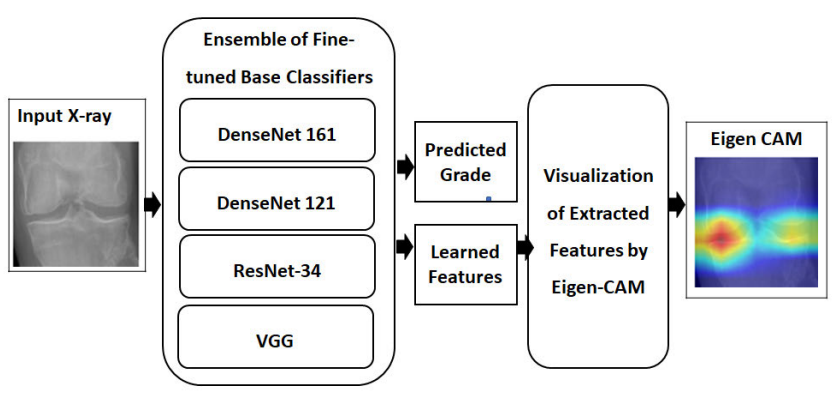
\includegraphics[width=0.8\textwidth]{figs/tariq2023.png}
    \caption{Metodologia proposta por \citeonline{Tariq2023}.}
    \label{fig:tariq2023}
\end{figure}

Ainda em 2023, \citeonline{Mohammed2023} utilizaram seis modelos pré-treinados de RNC (VGG-16, VGG-19, ResNet-101, MobileNetV2, InceptionResNetV2 e DenseNet-121) para diagnosticar a OA de joelho, considerando vários cenários de teste, como a classificação binária e o nível de severidade com três e cinco classes (\autoref{fig:mohammed2023}). O destaque do estudo foi a experimentação dos modelos em diferentes cenários, modelando tanto a detecção, quanto a própria classificação da OA, através do agrupamento das radiografias. O modelo ResNet-101 registrou as acurácias máximas com cinco, duas e três classes, sendo 69\%, 83\% e 89\%, respectivamente.

\begin{figure}[!htbp]
    \centering
    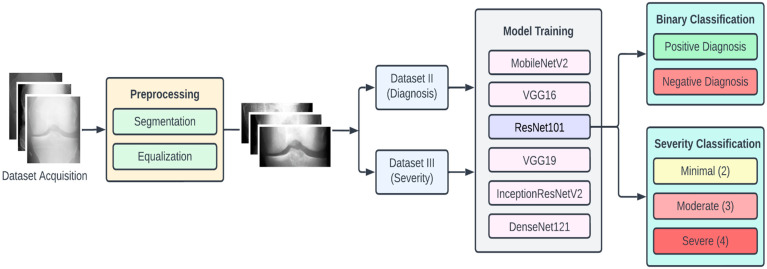
\includegraphics[width=\textwidth]{figs/mohammed2023.jpg}
    \caption{Metodologia proposta por \citeonline{Mohammed2023}.}
    \label{fig:mohammed2023}
\end{figure}

Partindo para a introdução de um modelo customizado, os autores brasileiros \citeonline{domingues2023} propuseram um modelo de RNC baseado na arquitetura DenseNet-161, treinado com um conjunto de radiografias obtidas do Estudo Longitudinal de Saúde do Adulto Musculoesquelético (ELSA-Brasil Musculoesquelético), para a classificação binária automática da OA de joelho (\autoref{fig:domingues2023}). Eles aplicaram diversas técnicas de pré-processamento, como rotação, desfoque gaussiano e inversão horizontal, e alcançaram uma AUC de 0,866 (IC 95\%: 0,842-0,882), considerando uma média entre os subconjuntos de treino e teste. O modelo também pode ser calibrado por meio do ajuste de limiares para alcançar uma acurácia máxima de 90,7\% e uma sensibilidade de 93,8\%.

\begin{figure}[!htbp]
    \centering
    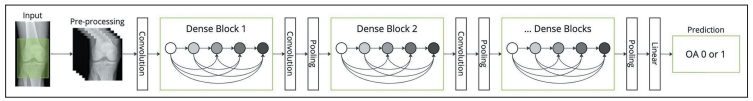
\includegraphics[width=\textwidth]{figs/domingues2023.png}
    \caption{Metodologia proposta por \citeonline{domingues2023}.}
    \label{fig:domingues2023}
\end{figure}

\citeonline{Cueva2022} desenvolveram um sistema de diagnóstico por computação assistida (CAD) utilizando a técnica de ajuste fino do modelo ResNet-34 para detectar OA nos dois joelhos simultaneamente (\autoref{fig:cueva2022}). Os autores resolveram o problema de desequilíbrio do conjunto de dados por meio de técnicas de \textit{oversampling} e \textit{data augmentation}, como rotação aleatória e variação de cor. O modelo alcançou uma acurácia média de 61,71\% em múltiplas classes, com melhor desempenho para as classes KL-0, KL-3 e KL-4 em comparação com KL-1 e KL-2 devido às sutis diferenças nos estágios intermediários.

\begin{figure}[!htbp]
    \centering
    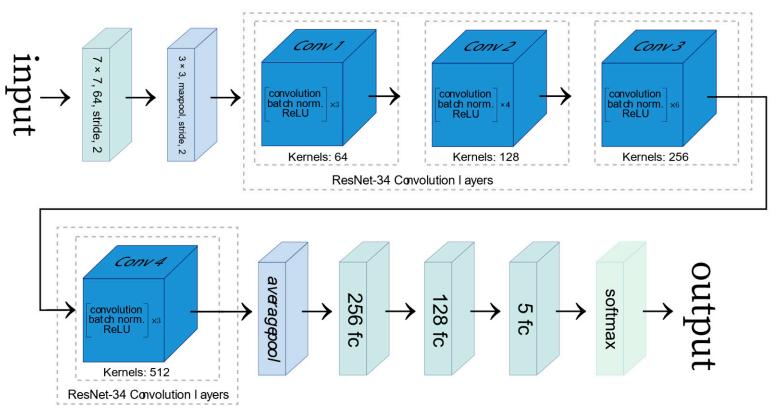
\includegraphics[width=\textwidth]{figs/cueva2022.png}
    \caption{Metodologia proposta por \citeonline{Cueva2022}.}
    \label{fig:cueva2022}
\end{figure}

Utilizando uma outra abordagem, \citeonline{yeoh2023} investigaram o uso de redes neurais convolucionais 3D para a detecção binária de OA de joelho a partir de imagens de ressonância magnética 3D. O estudo também utilizou transferência de aprendizado, transformando pesos de modelos pré-treinados em 2D para 3D. A abordagem permitiu capturar informações espaciais nas três dimensões, resultando em uma acurácia de 87,5\% e um F1-score de 0,871 para o melhor modelo, o ResNet-34.

Com a introdução dos ViTs, novas possibilidades surgiram para trabalhar o mesmo problema, oferecendo uma alternativa às RNCs, por vezes superando-as em tarefas de classificação de imagens. Em 2023, \citeonline{sekhri2023} introduziram uma abordagem utilizando o Swin Transformer para previsão da severidade da OA de joelho. Para lidar com a alta similaridade entre os graus adjacentes da escala KL, eles implementaram uma arquitetura de múltiplas previsões composta por cinco redes perceptron multicamadas (MLP), cada uma dedicada a prever um grau específico de KL. Além disso, para reduzir o desvio de dados entre os conjuntos de dados (OAI e MOST), congelaram as camadas MLP após o treinamento inicial em um conjunto de dados e continuaram treinando o extrator de características em outro para alinhar os espaços representacionais latentes. Essa abordagem alcançou acurácia de 70,17\% e F1-score de 0,67 no conjunto de dados OAI, superando os métodos existentes do estado da arte.

\begin{figure}[!htbp]
    \centering
    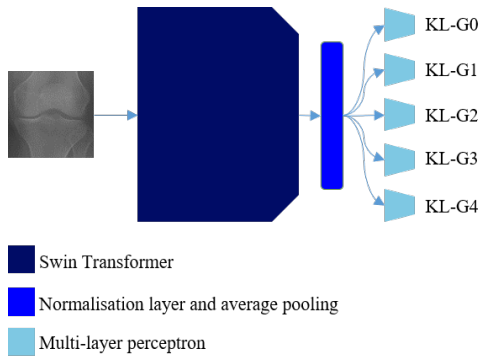
\includegraphics[width=0.7\textwidth]{figs/sekhri2023.png}
    \caption{Metodologia proposta por \citeonline{sekhri2023}.}
    \label{fig:sekhri2023}
\end{figure}

\citeonline{Wang_2024} criaram um modelo baseado em ViT para a detecção precoce da OA de joelho, focando na distinção entre o grau KL-0 e KL-2 (\autoref{fig:wang2024}). A metodologia incorporou três inovações principais:

\begin{itemize}
    \item \textit{Selective Shuffled Position Embedding} (SSPE): Ao fixar o posicionamento de ``patches-chave'' (regiões com características de grau KL) e embaralhar os demais, o modelo foi forçado a focar nas áreas críticas afetadas pela OA.
    \item Estratégia de troca de patches-chave: Como a técnica de aumento de dados, patches-chave de imagens candidatas foram trocados com a imagem alvo para gerar sequências de entrada diversas.
    \item Função de perda híbrida: Uma combinação de \textit{Label Smoothing Cross-Entropy} (LSCE) para sequências mistas de grau KL e \textit{cross-entropy} (CE) para sequências completas de grau KL foi otimizada para melhorar a generalização do modelo.
\end{itemize}

Essas estratégias resultaram em uma melhoria notável no desempenho de classificação, com o modelo alcançando uma acurácia de 89,80\%.

\begin{figure}[!htbp]
    \centering
    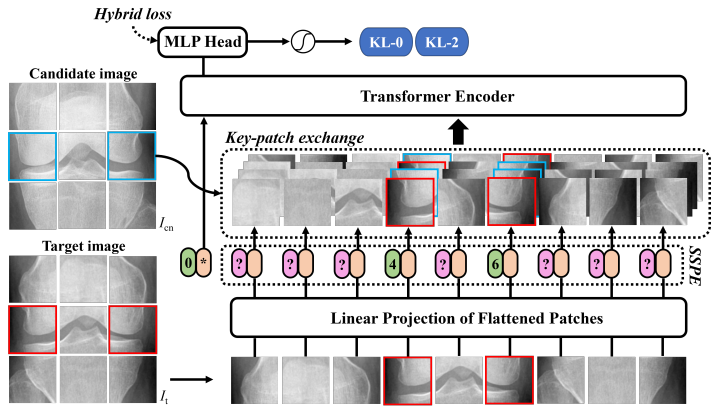
\includegraphics[width=\textwidth]{figs/wang2024.png}
    \caption{Metodologia proposta por \citeonline{Wang_2024}.}
    \label{fig:wang2024}
\end{figure}

Seguindo uma linha semelhante a este estudo, \citeonline{apon2024} conduziram uma análise comparativa entre modelos ViT pré-existentes (DaViT, GCViT, MaxViT) e RNCs tradicionais (\autoref{fig:apon2024}). Eles destacaram as forças arquitetônicas do DaViT com auto-atenção dupla, do GCViT com auto-atenção de contexto global e do MaxViT com atenção multi-eixo. Esses modelos ViT se destacaram com as melhores métricas, alcançando uma acurácia máxima de 66,14\%, precisão de 0,703, revocação de 0,614 e AUC superior a 0,835, superando consistentemente as RNCs (com acurácia entre 55-65\%).

\begin{figure}[!htbp]
    \centering
    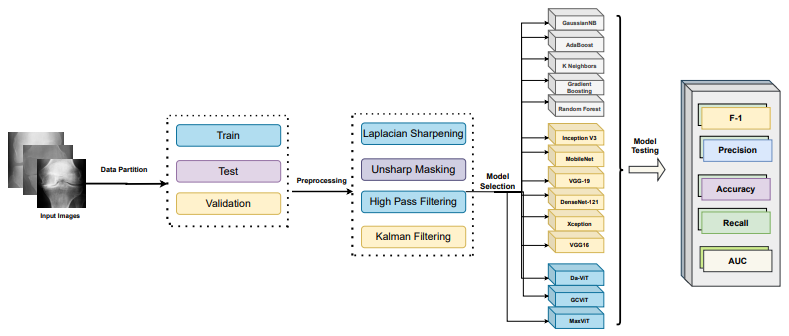
\includegraphics[width=\textwidth]{figs/apon2024.png}
    \caption{Metodologia proposta por \citeonline{apon2024}.}
    \label{fig:apon2024}
\end{figure}
% \chapter{Materiais e Métodos}\label{cap:ferramentas}

\lipsum[43-45]

\section{Considerações Finais}

\lipsum[23]


% PARTE
% \part{Proposta}
\chapter{Metodologia}\label{cap:proposta}

Esta seção descreve a metodologia proposta para a tarefa de classificação da OA de joelho a partir de radiografias. A principal abordagem desta pesquisa consiste no uso de \textit{transfer learning} para aproveitar o conhecimento já obtido por modelos pré-treinados e melhorar a performance da predição final.

\section{Coleta de dados}

A seleção e coleta de dados constituem etapas iniciais fundamentais no desenvolvimento de modelos de aprendizado profundo. Nesse estudo, o conjunto de dados (ou \textit{dataset} do inglês) foi obtido por meio da plataforma Kaggle \citep{dataset-kaggle}, amplamente reconhecida por disponibilizar dados de alta qualidade e de acesso público para fins acadêmicos. O \textit{dataset} escolhido baseia-se na Osteoarthritis Initiative (OAI) e contém 9.786 radiografias de joelho rotuladas com suas respectivas classificações de severidade da OA, seguindo o sistema de Kellgren-Lawrence (\autoref{tabela-kl}). A escolha desta fonte deve-se à sua ampla utilização na plataforma e na literatura \citep{Tariq2023, Mohammed2023}, além do volume de imagens, fornecendo uma base sólida e representativa para o treinamento e avaliação dos modelos propostos. Um resumo do \textit{dataset} é apresentado na \autoref{dataset-summary}.

\begin{table}[ht]
    \centering
    \begin{tabular}{|c|c|c|c|}
        \hline
        \textbf{Classe KL} & \textbf{Descrição} & \textbf{Total de imagens} & \textbf{\% do total} \\
        \hline
        0 & saudável & 3857 & 40\% \\
        1 & duvidoso & 1770 & 18\% \\
        2 & mínimo & 2578 & 26\% \\
        3 & moderado & 1286 & 13\% \\
        4 & severo & 295 & 3\% \\
        \hline
        \textbf{Total} & - & 9786 & 100\% \\
        \hline
    \end{tabular}
    \caption{Número de radiografias por classe KL no conjunto de dados original.}
    \label{dataset-summary}
\end{table}

Todas as imagens possuem resolução de 224x224 pixels e estão no formato PNG. As imagens foram agrupadas em subconjuntos de treino, teste, validação e calibração, com uma proporção de 7:1:1:1. O conjunto de treino é utilizado para treinar os modelos, o conjunto de validação é usado para ajustar os hiperparâmetros e monitorar o desempenho do modelo durante o treinamento, o conjunto de teste é utilizado para avaliar o desempenho final do modelo e verificar sua capacidade de generalização em dados novos, e o conjunto de calibração é usado para aplicar a estratégia de predição conformal, discutida na \autoref{sec:conformal-prediction}. A distribuição das imagens por subconjunto de dados pode ser visualizada na \autoref{dataset-distribuition}.

\begin{figure}[ht]
    \centering
    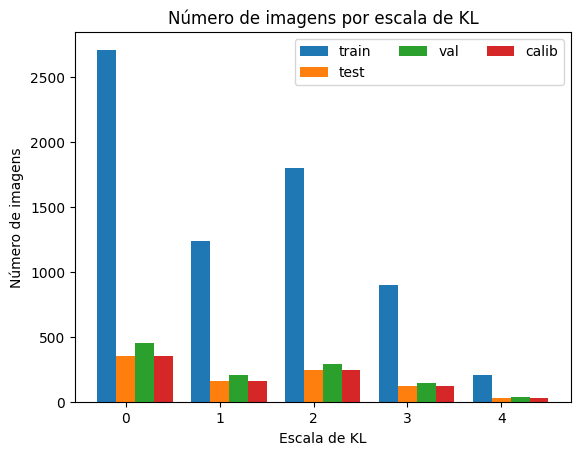
\includegraphics[width=0.7\linewidth]{figs/dataset-class-distribution.png}
    \caption{Distribuição das radiografias por classe KL nos subconjuntos de treino, teste, validação e calibração.}
    \label{dataset-distribuition}
\end{figure}

Com o objetivo de explorar diferentes abordagens para a classificação da severidade da OA de joelho, foram derivados, a partir do \textit{dataset} original contendo cinco classes, três novos conjuntos de dados: com 4, 3 e 2 classes. O conjunto com 4 classes foi construído por meio da exclusão da classe 1 (duvidosa), com a finalidade de simplificar o problema de classificação. O conjunto com 3 classes foi obtido pela remoção das classes 0 e 1 (respectivamente, saudável e duvidosa), resultando em um subconjunto composto apenas pelas instâncias que apresentavam algum grau de severidade (mínima, moderada ou severa). Por fim, o conjunto com 2 classes foi gerado ao se agrupar as classes 0 e 1, representando a ausência de OA, e as classes 2, 3 e 4, representando a presença de OA, formando, assim, um conjunto de dados binário.

\section{Pré-processamento das imagens}

A etapa de pré-processamento é essencial para garantir que as imagens estejam em um formato adequado para o treinamento dos modelos. Neste estudo, o pré-processamento das radiografias foi dividido em duas etapas: pré-processamento geral e pré-processamento específico para cada modelo. O pré-processamento geral, realizado antes do treinamento, inclui técnicas como equalização de histograma e filtro gaussiano. Já o pré-processamento específico para cada modelo, realizado durante o treinamento, envolve a adaptação das imagens às exigências de entrada dos modelos selecionados, como redimensionamento e normalização dos valores dos pixels. Além disso, o aumento de dados foi aplicado para expandir a variabilidade do conjunto de dados e mitigar o efeito do desbalanceamento entre as classes.

\subsection{Equalização de Histograma}

A equalização de histograma foi utilizada como técnica de pré-processamento com o intuito de melhorar o contraste das radiografias coletadas do conjunto original. Esse método redistribuiu os níveis de intensidade dos pixels de forma a abranger a maior faixa de valores possíveis, aumentando a separabilidade entre as regiões mais claras e mais escuras da radiografia. Em particular, essa técnica foi útil para realçar o contraste das estruturas ósseas e o espaço articular do joelho, assim como alterações ósseas sutis que podem ser indicativas de OA.

A aplicação da equalização de histograma foi realizada utilizando a biblioteca OpenCV \citep{opencv} do Python. A \autoref{fig:histogram-equalization}(a) ilustra uma radiografia original do joelho, enquanto a \autoref{fig:histogram-equalization}(b) mostra a mesma radiografia após a equalização de histograma. É possível observar que a equalização melhorou o contraste da imagem, tornando as estruturas ósseas mais visíveis. As respectivas distribuições de intensidade dos pixels antes e depois da equalização são apresentadas na \autoref{fig:histogram-equalization-histogram}.

\begin{figure}
    \centering
    \begin{tabular}{@{}c@{}}
        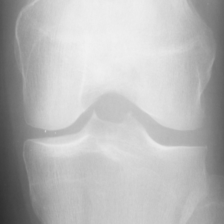
\includegraphics[width=0.45\textwidth]{figs/imagem-nao-equalizada.png} \\[\abovecaptionskip]
        \small (a) Radiografia original do joelho.
    \end{tabular}
    \hfill
    \begin{tabular}{@{}c@{}}
        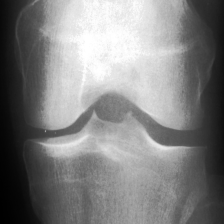
\includegraphics[width=0.45\textwidth]{figs/image-equalizada.png} \\[\abovecaptionskip]
        \small (b) Radiografia após equalização de histograma.
    \end{tabular}
    \caption{Exemplo de equalização de histograma aplicada a uma radiografia de joelho.}
    \label{fig:histogram-equalization}
\end{figure}

\begin{figure}
    \centering
    \begin{tabular}{@{}c@{}}
        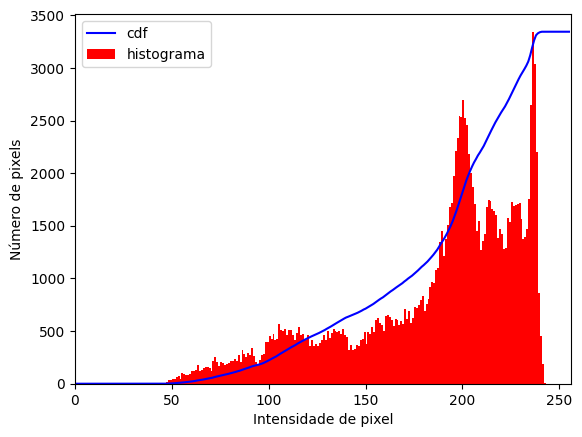
\includegraphics[width=0.45\textwidth]{figs/histograma-imagem-nao-equalizada.png} \\[\abovecaptionskip]
        \small (a) Histograma da radiografia original.
    \end{tabular}
    \hfill
    \begin{tabular}{@{}c@{}}
        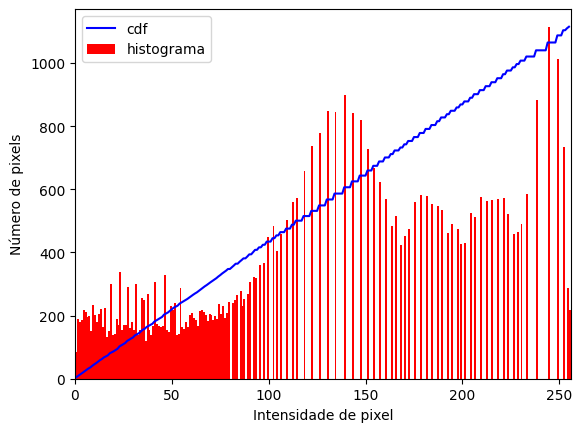
\includegraphics[width=0.45\textwidth]{figs/histograma-imagem-equalizada.png} \\[\abovecaptionskip]
        \small (b) Histograma da radiografia após equalização.
    \end{tabular}
    \caption{Distribuições de intensidade dos pixels antes e depois da equalização de histograma.}
    \label{fig:histogram-equalization-histogram}
\end{figure}

\subsection{Normalização}

A normalização das radiografias consistiu em uma etapa fundamental do pré-processamento, com o objetivo de padronizar a escala dos valores dos pixels e, assim, facilitar o aprendizado pelos modelos. Essa técnica foi aplicada convertendo os valores de intensidade dos pixels, originalmente na faixa de 0 a 255, para uma faixa padronizada entre 0 e 1.

Neste estudo, a normalização foi implementada em todos os subconjuntos de dados utilizando a função \texttt{transforms.Normalize} da biblioteca PyTorch \citep{pytorch}, que aplica a normalização em cada canal (RGB), subtraindo a média e dividindo pelo desvio padrão. Para modelos baseados em arquiteturas tradicionais, como ResNet e VGG, utilizaram-se os valores convencionais:

\begin{itemize}
    \item Média: 0.485, 0.456 e 0.406
    \item Desvio padrão: 0.229, 0.224 e 0.225
\end{itemize}

Para modelos baseados em ViTs, como o DeiT e o Swin Transformer, foram utilizados os valores de normalização específicos para esses modelos, obtidos diretamente do objeto \texttt{processor}, utilizando a função \texttt{processor.image\_mean} e \texttt{processor.image\_std}, garantindo a compatibilidade com o pré-processamento original desses modelos.

\subsection{Aumento de dados}

Com o objetivo de melhorar a generalização dos modelos e reduzir o risco de \textit{overfitting}, foi aplicado o aumento de dados (\textit{data augmentation}) nas radiografias durante o treinamento dos modelos.

A técnica consistiu na aplicação de transformações geométricas simples nas imagens do conjunto de treinamento, de forma a simular variações naturais que poderiam ocorrer nas radiografias. As transformações incluíram a inversão horizontal (reflexão), com probabilidade de 50\%, e rotações aleatórias limitadas a um intervalo de -10 a 10 graus.

Antes das transformações, as imagens foram redimensionadas para o tamanho esperado pelo modelo, definido como 224x224 pixels para todos os modelos, exceto para o modelo InceptionV3, que requer imagens de 299x299 pixels.

\subsection{Subamostragem}

Como pode ser observado na \autoref{dataset-summary}, o conjunto de dados original apresenta um desbalanceamento significativo entre as classes, com a classe 0 (saudável) representando 40\% do total de imagens e a classe 4 (severo) apenas 3\%. Para lidar com esse desbalanceamento, além do aumento de dados, foi aplicada a técnica de subamostragem (\textit{undersampling}) nas classes majoritárias e reduzindo o número de imagens dessas classes, equilibrando sua proporção em relação às classes minoritárias.

A subamostragem foi aplicada apenas no conjunto de treinamento, de modo a não comprometer a representatividade das distribuições no conjunto de validação, testes e calibração. A técnica consistiu na seleção aleatória de um subconjunto das amostras das classes até um limite definido de 1.700 imagens por classe. Esse limite foi escolhido com base na classe 2 (mínima), que possui o maior número de imagens entre as classes com severidade, garantindo que todas as classes fossem representadas de forma equilibrada no conjunto de treinamento.

Embora essa estratégia possa levar à perda de informações potencialmente úteis, ela ajuda a reduzir o viés do modelo em direção às classes majoritárias e melhora sua capacidade de aprender padrões relevantes em todas as classes.

\section{Treinamento dos modelos}

A técnica de \textit{transfer learning} foi aplicada no treinamento dos modelos de classificação da OA de joelho com o objetivo de reaproveitar os pesos dos modelos pré-treinados e acelear o processo de convergência. Esse processo envolveu o uso de modelos pré-treinados no conjunto de dados ImageNet 1K \citep{Russakovsky2015}, onde tais modelos foram treinados para classificar imagens em 1.000 categorias distintas. O uso deste método de treinamento foi especialmente útil para este estudo, pois o conjunto de dados de radiografias de joelho é limitado em tamanho, o que poderia dificultar a capacidade dos modelos de aprender padrões significativos nas imagens.

O processo de treinamento dos modelos foi conduzido segundo um protocolo padronizado, assegurando robustez e reprodutibilidade. As arquiteturas foram inicializadas com pesos pré‑treinados obtidos de repositórios conhecidos, como o \textit{PyTorch} e o \textit{Hugging Face}, e tiveram sua camada de saída ajustada para corresponder ao número de classes da tarefa específica (5, 4, 3 ou 2 classes) e ao exigido pela função de perda empregada, sendo que para a \textit{CORN} o número de classes da camada de saída é subtraído em uma unidade. Além disso, adotou‑se a estratégia de não extração de características, na qual todas as camadas da rede permaneceram treináveis.

Cada modelo foi treinado com um \textit{batch size} de 28 imagens durante 60 épocas, utilizando uma política de embaralhamento aleatório dos dados. O otimizador Adam foi selecionado, com uma taxa de aprendizado inicial de 0,0001, e um \textit{scheduler} para diminuir a taxa de aprendizado em um fator de 10 a cada 5 épocas. Além disso, foi implementado um mecanismo de parada antecipada, com paciência de 5 épocas, baseado na perda de validação, para evitar o \textit{overfitting} dos modelos. A cada época, registraram‑se as métricas de desempenho em treinamento e validação; a taxa de aprendizado foi reduzida em ordem de magnitude a intervalos pré‑definidos, e o modelo de melhor acurácia de validação foi preservado.

Concluído o treinamento, recarregaram‑se os pesos do melhor modelo e traçaram‑se curvas de desempenho para análise visual da convergência. A avaliação final foi conduzida no conjunto de teste, produzindo relatório abrangente de métricas de classificação. A complexidade computacional de cada arquitetura, em termos de FLOPs e quantidade de parâmetros, foi estimada com auxílio da bibliteca \cite{ptflops}. Todos os resultados, incluindo métricas, tempo de execução e medidas de complexidade, foram armazenados em formato JSON para análise posterior.

Todos os modelos foram treinados no ambiente de computação em nuvem Google Colab, utilizando uma Nvidia T4 GPU com 16 GB de memória, adequada para a tarefa de ajuste fino em modelos pequenos. A escolha dessa plataforma foi motivada pela sua acessibilidade e capacidade de fornecer recursos computacionais adequados a um custo reduzido. A seguir, são apresentados os experimentos realizados com cada modelo, incluindo as métricas de desempenho obtidas e a análise dos resultados.

% PARTE
% \part{Parte Final}
\chapter{Resultados}\label{cap:resultados}

Esta pesquisa explora a transferência de aprendizado utilizando modelos pré-treinados no dataset ImageNet, aplicando ajuste fino para classificar o nível de severidade da osteoartrite de joelho com base na escala de Kellgren/Lawrence. O treinamento dos modelos foi realizado com a linguagem de programação Python, através de notebooks disponibilizados pela plataforma Google Colab, aproveitando os recursos computacionais de uma GPU T4 para acelerar o treino e a experimentação.

Para garantir a consistência entre os modelos, o treinamento foi realizado utilizando os mesmos hiperparâmetros. A classificação da osteoartrite de joelho foi organizada em cinco classes: KL 0, KL 1, KL 2, KL 3 e KL 4. O conjunto de dados foi dividido em 70\% para treinamento, 10\% para teste e 20\% para validação. Para mitigar possíveis vieses, a base de dados foi balanceada por meio de técnicas de \textit{undersampling} e \textit{oversampling}, limitando cada classe a um máximo de 1700 imagens, complementadas por estratégias de \textit{data augmentation}. O treinamento foi configurado com \textit{batches} de 28 imagens, executado ao longo de 30 épocas, com um \textit{early stopping} com 5 épocas de paciência para evitar \textit{overfitting}.

Dois conjuntos de treinamento foram conduzidos: no primeiro, a função de perda utilizada foi a \textit{crossentropy}, enquanto no segundo, foi substituída pela função de perda \textit{Conditional Ordinal Regression for Neural Networks} (CORN), com o objetivo de explorar sua adequação ao problema de classificação ordinal. Em ambos os casos, o otimizador adotado foi o Adam, configurado com uma taxa de aprendizado inicial de 0.0001, ajustada dinamicamente a cada 3 épocas.

A \autoref{tab:resultados} mostra a acurácia dos modelos de RNCs e ViTs treinados para a classificação da OA de joelho usando a função de perda \textit{crossentropy}. Em relação ao tempo de treinamento, é possível notar que o modelo mais rápido foi o ResNet-50, com um tempo de 11.29 segundos. Por outro lado, o modelo mais lento foi o DeiT, com um tempo de 79.5 segundos. Tais valores não necessariamente indicam que o modelo mais rápido é o pior, ou o contrário, mas é importante considerar o tempo de treinamento como um fator relevante ao escolher um modelo, especialmente se houver restrições de recursos computacionais. O tempo de treinamento mostrado varia, principalmente, com o número de épocas, já que modelos que levaram mais tempo são aqueles que tiveram a parada antecipada mais tarde, ou executaram as 30 épocas completas.

\begin{table}
    \centering
    \begin{tabular}{|c|c|c|c|c|c|c|c|}
        \hline
        \multirow{2}{*}{Modelo} & \multirow{2}{*}{Tempo (min)} & \multirow{2}{*}{Overall} & \multicolumn{5}{|c|}{Classe KL} \\ \cline{4-8}
        &  &  & 0 & 1 & 2 & 3 & 4 \\ \hline
        ResNet-34 & 14.85 & 0.7044 & 0.8146 & 0.3889 & 0.6680 & 0.8519 & 0.8246 \\ \hline
        ResNet-50 & 11.29 & 0.7248 & 0.8359 & 0.4475 & 0.6988 & 0.7942 & 0.8596 \\ \hline
        ResNet-101 & 18.81 & 0.7126 & 0.8031 & 0.4414 & 0.7029 & 0.7984 & 0.8596 \\ \hline
        VGG-16 & 51.33 & 0.6723 & 0.8588 & 0.2562 & 0.6783 & 0.8272 & 0.8421 \\ \hline
        VGG-19 & 23.21 & 0.6851 & 0.8217 & 0.2716 & 0.6906 & 0.7984 & 0.8246 \\ \hline
        DenseNet-121 & 24.48 & 0.7170 & 0.8616 & 0.2963 & 0.707 & 0.8477 & 0.8596 \\ \hline
        DenseNet-169 & 16.85 & 0.7319 & 0.8288 & 0.4043 & 0.7377 & 0.8477 & 0.8596 \\ \hline
        Inception-v3 & 16.45 & 0.7215 & 0.8017 & 0.4136 & 0.75 & 0.8148 & 0.8421 \\ \hline
        ViT-B & 43.07 & 0.6955 & 0.8046 & 0.3241 & 0.7029 & 0.823 & 0.8596 \\ \hline
        DeiT & 79.5 & 0.6862 & 0.7718 & 0.3488 & 0.6947 & 0.8354 & 0.8421 \\ \hline
        Swin & 17.88 & 0.6977 & 0.8388 & 0.3117 & 0.6824 & 0.8025 & 0.8421 \\ \hline
    \end{tabular}
    \caption{Desempenho dos modelos de RNCs e ViTs na classificação da OA de joelho usando a função de perda \textit{crossentropy}.}
    \label{tab:resultados}
\end{table}

Quanto à acurácia geral (\textit{overall}), todos os modelos apresentaram resultados razoavelmente bons, com valores variando de 0.6723 a 0.7319. Isso indica que todos os modelos foram capazes de aprender padrões relevantes para a classificação da OA de joelho. No entanto, é importante notar que o modelo DenseNet-169 obteve a maior acurácia geral, com um valor de 0.7319. Isso sugere que arquiteturas de RNCs densamente conectadas podem ser muito eficazes na extração de características relevantes em imagens médicas como radiografias de joelho. Além disso, os modelos de conexões residuais (ResNet) também apresentaram resultados competitivos, com acurácias gerais variando de 0.7044 a 0.7248, onde o ResNet-50 obteve a maior acurácia dentre eles e com o menor tempo de treinamento, oferecendo um bom equilíbrio entre generalização do modelo e custo computacional.

Por outro lado, os modelos da família VGG (VGG-16 e VGG-19) apresentaram acurácias gerais mais baixas, variando de 0.6723 a 0.6851, o que sugere que essas arquiteturas mais simples podem não ser tão eficazes na extração de características complexas em radiografias de joelho. Embora fosse esperado que esses modelos tivessem desempenho inferior em relação aos modelos ResNet, devido à sua profundidade, os resultados indicam que esses modelos são capazes de aprender padrões relevantes e ter uma menor probabilidade de \textit{overfitting}, como observado no tempo de treinamento do VGG-16, que foi maior que a maioria dos modelos justamente por não ter parada antecipada em virtude da queda do erro no conjunto de validação.

O GoogLeNet, com sua arquitetura Inception (versão 3), permitiu que o modelo tivesse uma acurácia geral de 0.7215, indicando que o modelo pode ser eficaz na extração de características relevantes e superar a maioria dos modelos de RNCs. Esse comportamento pode ser justificado pelo uso de uma técnica chamada de "bottleneck" ou "redução de dimensionalidade", que reduz a quantidade de parâmetros e a complexidade computacional do modelo, sem comprometer significativamente o desempenho.

Os modelos de transformers, por sua vez, apresentaram acurácias gerais variando de 0.6862 a 0.7215, indicando que essas arquiteturas podem ser eficazes, mas talvez não sejam tão eficientes quanto os modelos de RNCs. O modelo Swin Transformer obteve a maior acurácia geral entre os modelos de transformers, com um valor de 0.6977, sugerindo que a abordagem hierárquica de atenção pode ser eficaz na extração de características relevantes em radiografias de joelho.

Entretanto, é importante notar que a acurácia para a classe KL 1 foi baixa para todos os modelos, variando de 0.2562 e 0.4475. Isso indica que a classificação da OA de joelho no estágio 1 (duvidoso) pode ser mais desafiadora, possivelmente devido à semelhança visual com as classes adjacentes KL 0 e KL 2. Esse resultado pode ser observado na \autoref{confusion-matrix-resnet50}, que mostra a matriz de confusão do modelo ResNet-50. A classe KL 1 tem a menor acurácia dentre todas as classes, o que reflete o desafio na classificação dessa classe devido ao nível de detalhe ou até mesmo incoerência no rotulação das imagens do dataset.

\begin{figure}[h]
    \centering
    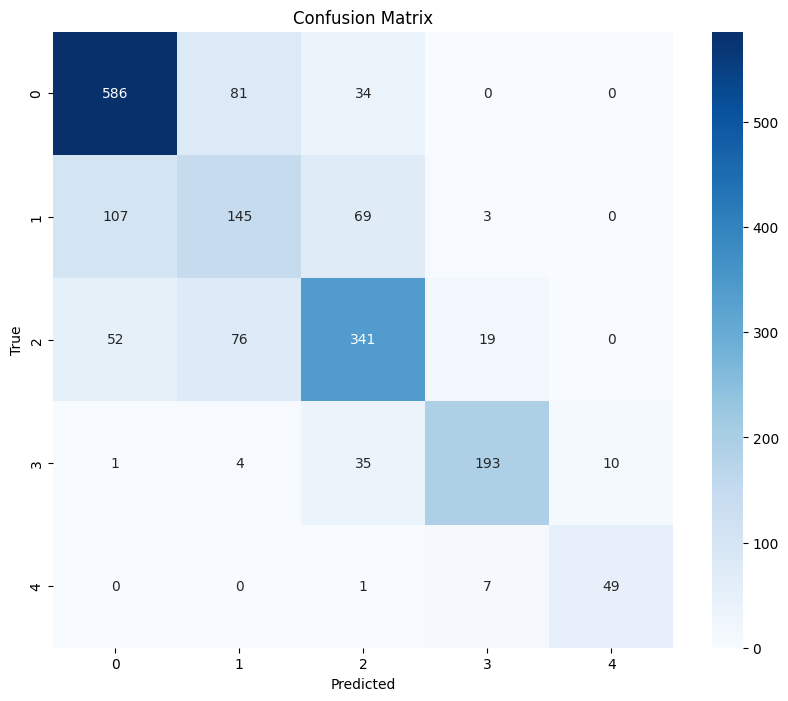
\includegraphics[width=\linewidth]{figs/confusion-matrix-resnet50.png}
    \caption{Matriz de confusão do modelo ResNet-50.}
    \label{confusion-matrix-resnet50}
\end{figure}

Em resumo, os modelos ResNet-50 e DenseNet-169 se destacaram em termos de tempo de treinamento e acurácia geral, respectivamente. No entanto, é importante considerar as características de cada classe ao escolher um modelo, pois diferentes modelos podem ter desempenhos diferentes para cada classe.

A \autoref{tab:resultados-corn} apresenta os resultados dos modelos de RNCs e ViTs treinados para a classificação da OA de joelho usando a função de perda CORN. Em relação ao tempo de treinamento, não houve uma mudança significativa comparado com a função de perda \textit{crossentropy}. O modelo mais rápido foi, novamente, o ResNet-50, com um tempo de 10.32 segundos, enquanto o modelo mais lento foi o Swin Transformer, com um tempo de 35.58 segundos. Em relação à acurácia geral, os resultados variaram de 0.6546 a 0.7181, indicando que a função de perda CORN pode ser eficaz na classificação da OA de joelho, mas não necessariamente supera a função de perda \textit{crossentropy}. Isso é justificado pelo fato de que a função de perda CORN é mais adequada quando o modelo faz predições mais afastadas do rótulo real, o que não foi evidenciado ao observar as matrizes de confusão dos modelos.

\begin{table}
    \centering
    \begin{tabular}{|c|c|c|c|c|c|c|c|}
        \hline
        \multirow{2}{*}{Modelo} & \multirow{2}{*}{Tempo} & \multirow{2}{*}{Overall} & \multicolumn{5}{|c|}{Classe KL} \\ \cline{4-8}
        &  &  & 0 & 1 & 2 & 3 & 4 \\ \hline
        ResNet-34 & 14.93 & 0.6895 & 0.7518 & 0.5586 & 0.6107 & 0.8107 & 0.8246 \\ \hline
        ResNet-50 & 10.32 & 0.7181 & 0.796 & 0.5031 & 0.6824 & 0.823 & 0.8421 \\ \hline
        ResNet-101 & 16.17 & 0.6994 & 0.7418 & 0.4506 & 0.707 & 0.8519 & 0.8772 \\ \hline
        VGG-16 & 19.29 & 0.6762 & 0.7646 & 0.358 & 0.6824 & 0.7984 & 0.8246 \\ \hline
        VGG-19 & 24.05 & 0.6669 & 0.7974 & 0.3549 & 0.6066 & 0.7901 & 0.8246 \\ \hline
        DenseNet-121 & 10.62 & 0.6911 & 0.729 & 0.4444 & 0.7172 & 0.8272 & 0.8246 \\ \hline
        DenseNet-169 & 13.75 & 0.717 & 0.7874 & 0.5833 & 0.6393 & 0.8148 & 0.8596 \\ \hline
        Inception-v3 & 17.09 & 0.701 & 0.7932 & 0.5093 & 0.6639 & 0.7325 & 0.8421 \\ \hline
        ViT-B & 36.97 & 0.6817 & 0.7447 & 0.4815 & 0.6393 & 0.8066 & 0.8772 \\ \hline
        DeiT & 34.73 & 0.6602 & 0.7047 & 0.4877 & 0.6209 & 0.7984 & 0.8421 \\ \hline
        Swin & 35.58 & 0.6546 & 0.7803 & 0.4658 & 0.6722 & 0.8395 & 0.7894 \\ \hline
    \end{tabular}
    \caption{Desempenho dos modelos de RNCs e ViTs na classificação da OA de joelho usando a função da perda CORN.}
    \label{tab:resultados-corn}
    \end{table}

No entanto, é importante notar que o modelo ResNet-50 obteve a maior acurácia geral, com um valor de 0.7181, superando os demais modelos, inclusive o modelo DenseNet-169, que obteve a maior acurácia geral com a função de perda \textit{crossentropy}. Isso sugere que a função de perda CORN pode ser eficaz em arquiteturas de RNCs, especialmente aquelas com conexões residuais. Entretanto, o modelo DenseNet-169 foi quem obteve a maior acurácia para a classe KL 1, com um valor de 0.5833, que é a classe mais desafiadora de ser classificada, como observado anteriormente.
% \chapter{Conclusão}\label{cap:conclusao}

Este trabalho se propôs a realizar uma análise comparativa abrangente entre arquiteturas de redes neurais convolucionais (RNCs) e vision transformers (ViTs) para a tarefa de classificação da severidade da osteoartrite (OA) de joelho, utilizando a escala de Kellgren/Lawrence. Diante da subjetividade e do tempo demandado pelo diagnóstico manual, o objetivo central foi identificar os modelos mais robustos, eficientes e confiáveis, empregando uma avaliação com diferentes variáveis que incluiu desempenho preditivo, custo computacional, quantificação de incerteza e interpretabilidade.

A investigação sistemática das treze arquiteturas revelou conclusões claras e significativas. Os modelos da família DenseNet se destacaram como os de melhor desempenho geral. O DenseNet-169 alcançou a maior acurácia (78,85\%), enquanto o DenseNet-121 obteve o maior QWK (0,8878), demonstrando a melhor performance preditiva na tarefa de classificação ordinal.

A comparação entre as funções de perda de entropia cruzada e CORN evidenciou uma compensação fundamental. Enquanto a entropia cruzada maximizou a acurácia, a função CORN consistentemente melhorou o QWK, minimizando a gravidade dos erros de classificação. Adicionalmente, a análise com a predição conformal mostrou que a abordagem com CORN gera conjuntos de predição drasticamente mais informativos e úteis para a prática clínica.

A análise da eficiência computacional apresentou uma expressiva vantagem de eficiência das RNCs sobre os ViTs. Modelos como DenseNet-121 e ResNet-50 foram de quatro a cinco vezes mais rápidos em inferência do que os ViTs de alto desempenho, como DaViT-B e Swin-B. Esse resultado sublinha um desafio prático para a implantação de ViTs em ambientes clínicos que demandam baixo custo e alta velocidade.

A análise com Grad-CAM confirmou que os modelos de melhor desempenho basearam suas decisões em marcadores patológicos clinicamente relevantes, como o espaço articular e osteófitos. Também foram identificadas ``estratégias visuais'' distintas, com as RNCs produzindo ativações mais focadas e os ViTs, mais contextuais.

Apesar do rigor metodológico, este trabalho possui algumas limitações que devem ser reconhecidas. O estudo foi conduzido num único conjunto de dados público com um desbalanceamento claro. Além disso, a anaĺise se baseou apenas em imagens estáticas, sem qualquer informação extra sobre os pacientes. Trabalhos futuros podem explorar outros conjuntos de dados para garantir a generalização dos resultados, integrar com um estudo longitudinal que acompanhasse a progressão da OA ao longo do tempo, além de otimizar as arquiteturas com estratégias de \textit{grid-searching} e \textit{ensemble}, combinando a saída dos melhores modelos para determinar a classe KL.

Este trabalho demonstrou com sucesso que modelos de aprendizado profundo, em particular as RNCs e ViTs, são capazes de classificar a severidade da OA de joelho com alta acurácia e confiabilidade. Mais importante, o estudo evidenciou que uma avaliação completa deve ir além da acurácia, considerando a relevância clínica do erro, a eficiência computacional e a interpretabilidade. Assim, o estudo fornece um \textit{benchmark} sólido para o desenvolvimento de futuras ferramentas de IA que possam auxiliar profissionais da saúde no diagnóstico e manejo da OA de joelho.

% ----------------------------------------------------------
% ELEMENTOS PÓS-TEXTUAIS (Referências, Glossário, Apêndices)
% ----------------------------------------------------------
\postextual

% Referências bibliográficas
\bibliography{bibliografia}

% Glossário (Consulte o manual)
%\glossary

% Apêndices
% % ----------------------------------------------------------
% Apêndices
% ----------------------------------------------------------

% ---
% Inicia os apêndices
% ---
\begin{apendicesenv}

% Imprime uma página indicando o início dos apêndices
\partapendices

% ----------------------------------------------------------
\chapter{Resultados Suplementares}
% ----------------------------------------------------------

Como complemento à análise principal, foram conduzidos experimentos para avaliar o desempenho dos modelos na tarefa de classificar a OA de joelho em 4, 3 e 2 classes, através da manipulação das imagens do conjunto de dados.

\section{Classificação em 4 Classes}
\label{apendice:resultados_4_classes}

Inicialmente, foi realizado um experimento para a tarefa de classificação em 4 classes, excluindo a classe KL-1 (``duvidoso''). O objetivo foi investigar o impacto da remoção desta classe, identificada como ambígua no desempenho geral das arquiteturas.

A exclusão da classe KL-1 resultou em um aumento substancial e generalizado no desempenho de todos os modelos, validando a hipótese de que a ambiguidade desta classe era um dos principais desafios para a tarefa de classificação. A \autoref{tab:overall_metrics_4_classes} resume as métricas de desempenho para os modelos mais relevantes neste cenário.

O resultado mais notável foi o aumento significativo na performance. O modelo GCViT-B, treinado com a função de perda CORN, alcançou uma acurácia de 90,08\%, um QWK de 0,9311 e um MAE de 0,1635, estabelecendo-se como o modelo de melhor desempenho neste cenário. Outros modelos, como o DaViT-B, também apresentaram resultados expressivos, com 89,28\% de acurácia e 0,9267 de QWK.

Diferentemente do cenário de 5 classes, onde os modelos da família DenseNet se destacaram, a remoção da classe ambígua permitiu que os ViTs, em particular o GCViT-B e o DaViT-B, demonstrassem seu pleno potencial, superando as RNCs em acurácia e QWK.

\begin{table}[!htbp]
    \centering
    \caption{Resumo das métricas gerais de desempenho para modelos selecionados no cenário de 4 classes.}
    \label{tab:overall_metrics_4_classes}
    \begin{tabular}{|l|l|c|c|c|}
        \hline
        \textbf{Modelo} & \textbf{Função de perda} & \textbf{Acurácia} & \textbf{QWK} & \textbf{MAE} \\
        \hline
        ResNet-50 & \text{CORN} & 87,67\% & 0,9146 & 0,2105 \\
        \hline
        DenseNet-121 & \text{CORN} & 88,20\% & 0,9153 & 0,1957 \\
        \hline
        DenseNet-169 & \text{CORN} & 88,34\% & 0,9192 & 0,2051 \\
        \hline
        Inception-v3 & \text{Entropia Cruzada} & 88,61\% & 0,9225 & 0,1917 \\
        \hline
        DaViT-B & \text{Entropia Cruzada} & 89,28\% & 0,9267 & 0,1783 \\
        \hline
        GCViT-B & \text{CORN} & \textbf{90,08\%} & \textbf{0,9311} & \textbf{0,1635} \\
        \hline
    \end{tabular}
\end{table}

\section{Classificação em 3 Classes}
\label{apendice:resultados_3_classes}

Um segundo experimento foi conduzido para avaliar a capacidade dos modelos em distinguir exclusivamente entre os diferentes estágios de severidade da OA, uma vez que a doença já está estabelecida. Para este fim, as classes KL-0 (saudável) e KL-1 (duvidoso) foram removidas, resultando em um problema de classificação com 3 classes: KL-2 (mínimo), KL-3 (moderado) e KL-4 (severo).

Essa simplificação do problema, focando apenas nos estágios da doença, resultou em um desempenho preditivo alto em todas as arquiteturas avaliadas. A \autoref{tab:overall_metrics_3_classes} resume as métricas de desempenho para os modelos mais relevantes neste cenário. O resultado mais interessante foi a alta acurácia e concordância ordinal alcançadas. O modelo Inception-v3, treinado com a entropia cruzada,, atingiu a maior acurácia de 94,43\% e o maior QWK de 0,9285. Ainda assim, os demais modelos tiveram uma ótima performance.

Estes resultados indicam que os modelos avaliados possuem uma alta capacidade não apenas para detectar a OA, mas também para diferenciar seus estágios de severidade, uma tarefa fundamental para o planejamento de tratamentos e o acompanhamento da progressão da doença.

\begin{table}[!htbp]
    \centering
    \caption{Resumo das métricas gerais de desempenho para modelos selecionados no cenário de 3 classes.}
    \label{tab:overall_metrics_3_classes}
    \begin{tabular}{|l|l|c|c|c|}
        \hline
        \textbf{Modelo} & \textbf{Função de perda} & \textbf{Acurácia} & \textbf{QWK} & \textbf{MAE} \\
        \hline
        ResNet-101 & \text{Entropia Cruzada} & 92,91\% & 0,9082 & 0,0709 \\
        \hline
        DenseNet-121 & \text{CORN} & 93,42\% & 0,9136 & 0,0658 \\
        \hline
        DaViT-B & \text{Entropia Cruzada} & 93,92\% & 0,9218 & 0,0608 \\
        \hline
        DenseNet-169 & \text{CORN} & 93,92\% & 0,9220 & 0,0608 \\
        \hline
        Inception-v3 & \text{Entropia Cruzada} & \textbf{94,43\%} & \textbf{0,9285} &  \textbf{0,0557} \\
        \hline
        GCViT-B & \text{Entropia Cruzada} & 93,16\% & 0,9110 & 0,0684 \\
        \hline
    \end{tabular}
\end{table}

\section{Classificação em 2 Classes}
\label{apendice:resultados_2_classes}

Finalmente, um terceiro experimento foi realizado para avaliar a capacidade dos modelos em uma tarefa de detecção binária, que possui grande relevância clínica para a triagem inicial de pacientes. Neste cenário, as classes KL-0 e KL-1 foram agrupadas para representar a ``ausência de OA'', enquanto as classes KL-2, KL-3 e KL-4 foram consolidadas para representar a ``presença de OA''.

Os resultados, resumidos na \autoref{tab:overall_metrics_2_classes}, indicam que todos os modelos foram capazes de realizar a detecção binária com um desempenho robusto, alcançando acurácias na faixa de 84\% a 87\%. Nesta formulação do problema, os ViTs demonstraram uma ligeira vantagem. O modelo GCViT-B (entropia cruzada) destacou-se com a maior acurácia, atingindo 87,10\%, além do maior QWK de 0,7374 e MAE de 0,1290, indicando a melhor concordância ajustada ao acaso. Logo em seguida, o MaxViT-T (CORN) também apresentou um excelente resultado, com 86,77\% de acurácia.

As diferenças de desempenho entre as funções de perda foram mínimas e inconsistentes neste cenário, o que é esperado, uma vez que para um problema de duas classes a formulação ordinal do CORN se aproxima da logística binária padrão.

\begin{table}[!htbp]
    \centering
    \caption{Resumo das métricas gerais de desempenho para modelos selecionados no cenário de classificação binária.}
    \label{tab:overall_metrics_2_classes}
    \begin{tabular}{|l|l|c|c|c|}
        \hline
        \textbf{Modelo} & \textbf{Função de perda} & \textbf{Acurácia} & \textbf{QWK} & \textbf{MAE} \\
        \hline
        ResNet-50 & \text{CORN} & 84,90\% & 0,6956 & 0,1510 \\
        \hline
        DenseNet-121 & \text{CORN} & 85,67\% & 0,6861 & 0,1433 \\
        \hline
        DenseNet-169 & \text{CORN} & 85,56\% & 0,7055 & 0,1444 \\
        \hline
        DaViT-B & \text{CORN} & 86,55\% & 0,7268 & 0,1345 \\
        \hline
        MaxViT-T & \text{CORN} & 86,77\% & 0,7300 & 0,1323 \\
        \hline
        GCViT-B & \text{Entropia Cruzada} & \textbf{87,10\%} & \textbf{0,7374} & \textbf{0,1290} \\
        \hline
    \end{tabular}
\end{table}

\end{apendicesenv}
% ---

% Anexos
% % ----------------------------------------------------------
% Apêndices
% ----------------------------------------------------------

% ---
% Inicia os anexos
% ---
\begin{anexosenv}

% Imprime uma página indicando o início dos anexos
\partanexos

% ---
\chapter{Nome do Primeiro Anexo}
% ---
\lipsum[30] % Texto qualquer. REMOVER!!

% ---
\chapter{Nome de Outro Anexo}
% ---

\lipsum[32] % Texto qualquer. REMOVER!!

\end{anexosenv}

% Índice remissivo (Consultar manual)
%\phantompart
%\printindex

\end{document}
